Per la pianificazione, sono stati individuati 5 periodi, scelti in base ai processi primari coinvolti. Ogni periodo contiene diverse attività. Nella pianificazione, verrà impiegata tale numerazione:
\begin{center}
	[\textbf{Periodo}].[\textbf{Attività}]
\end{center}
se le attività non vengono raggruppate,
\begin{center}
	[\textbf{Periodo}].[\textbf{Insieme di attività}].[\textbf{Attività}]
\end{center}
altrimenti.\\
La numerazione, sia per i periodi, sia per gli insiemi di attività, sia per le singole attività, è sequenziale.\\
Alla fine di ogni periodo, segue la tabella con le assegnazioni dei membri alle attività. Nella prima colonna di ogni tabella, si trovano le attività, indicate col numero assegnato. Nelle restanti, viene indicato a quale membro è stata affidata ciascuna attività tramite un $\bullet$ nella relativa colonna. I nominativi dei membri sono stati sostituiti con le prime tre lettere del cognome: BER (Bergo), BOR (Bortone), COS (Cosentino), MAR (Marcato), PEA (Peagno), PER (Peron), PET (Pettenuzzo).

\newpage
\subsection{Periodo di Avvio e di Analisi (2018-12-04 - 2018-02-09)}
		\subsubsection{Periodo di Avvio (2018-12-04 - 2018-12-17)}
		Nel periodo di avvio hanno luogo le seguenti attività:
		\begin{enumerate}[label = 1.\arabic*)]
			\item ricerca degli strumenti (2018-12-4 - 2018-12-14): tutti i membri del gruppo effettuano le ricerche sui possibili strumenti utili alle attività di avvio e di analisi dei requisiti;
			\item prima normazione (2018-12-5 - 2018-12-14): gli amministratori redigono le \textit{Norme di progetto} concordate per i processi di supporto e organizzativi;
			\item studio di fattibilità (2018-12-4 - 2018-12-8): gli analisti effettuano lo \textit{Studio di fattibilità} dei capitolati;
			\item pianificazione di progetto (2018-12-7 - 2018-12-13): il responsabile redige il \textit{Piano di progetto}, riportando modello di sviluppo, analisi dei rischi e la pianificazione per le prime attività dell'analisi dei requisiti;
			\item verifica dei documenti (2018-12-15 - 2018-12-16): i verificatori controllano se i documenti siano corretti.
		\end{enumerate}
		
	\subsubsection{Periodo di Analisi (2018-12-17 - 2018-02-09)}	
		\paragraph{Pianificazione (2018-12-17 - 2018-12-23)\\} Il periodo di analisi dei requisiti inizia con le attività di:
			\begin{enumerate}[label = 2.1.\arabic*)]
				\item pianificazione di progetto (2018-12-17 - 2018-12-21): il responsabile effettua il resoconto del periodo di avvio e pianifica in maniera più dettagliata le attività di analisi dei requisiti; 
				\item pianificazione della qualifica (2018-12-17 - 2018-12-21): i verificatori redigono il resoconto del periodo di avvio e gli amministratori effettuano i primi incrementi per il \textit{Piano di qualifica};
				\item normazione (2018-12-17 - 2018-12-21): gli amministratori redigono in maniera precisa e completa le \textit{Norme di progetto} per l'attività di analisi;
				\item verifica del \textit{Piano di progetto}, del \textit{Piano di qualifica} e delle \textit{Norme di progetto} (2018-12-21 - 2018-12-23).
			\end{enumerate}
		\paragraph{Analisi dei requisiti (2018-12-19 - 2018-02-09)\\} La parte centrale del periodo di analisi dei requisiti è costituita dalle attività di:
			\begin{enumerate}[label = 2.2.\arabic*)]
				\item analisi dei requisiti del sistema (2018-12-19 - 2018-12-27): gli analisti svolgono la prima analisi dei requisiti del sistema;
				\item incrementi al \textit{Piano di qualifica} (2018-12-26 - 2018-12-30): gli analisti introducono nel piano i test di sistema in base a quanto scaturito dall'analisi dei requisiti;
				\item verifica dell'analisi dei requisiti di sistema (2018-12-29 - 2018-12-31)
				\item verifica del \textit{Piano di qualifica} (2018-01-09 - 2019-01-03)
				\item incrementi all'analisi dei requisiti (2019-01-02 - 2019-01-08): gli analisti aggiungono degli incrementi all'analisi di sistema
				\item verifica degli incrementi all'analisi dei requisiti (2019-01-09 - 2019-01-11)
				\item incrementi al \textit{Piano di progetto} (2019-01-07 - 2019-01-10): il responsabile redige la parte di rendicontazione e consuntivo del \textit{Piano di progetto} da presentare alla Revisione dei Requisiti.
				\item incrementi al \textit{Piano di qualifica} (2019-01-07 - 2019-01-10): i verificatori redigono la parte di rendicontazione del \textit{Piano di qualifica} da presentare alla Revisione dei Requisiti, aggiungendo i risultati delle misurazioni effettuate, e gli analisti aggiungono i restanti test di sistema.
				\item verifica del \textit{Piano di progetto} e del \textit{Piano di qualifica} (2019-01-11 - 2019-01-12)
				\item preparazione alla presentazione (2019-01-15 - 2019-01-20);
				\item analisi dei requisiti software (2019-02-01 - 2019-02-05): gli analisti effettuano l'analisi dei requisiti software. Quest'attività è successiva al primo incremento di progettazione architetturale.
				\item verifica dell'analisi dei requisiti (2019-02-07 - 2019-02-09)				
			\end{enumerate}

	\begin{table}[h]
		\caption{Tabella delle assegnazioni per il periodo di avvio}
		\centering		
		\begin{tabular}{| >{\centering}p{1.5cm} | c | c | c | c | c | c | c |}
			\rowcolor{LightBlue}
			\textbf{\color{white}Numero attività} 
			& \textbf{\color{white}BER} 
			& \textbf{\color{white}BOR} 
			& \textbf{\color{white}COS} 
			& \textbf{\color{white}MAR} 
			& \textbf{\color{white}PEA} 
			& \textbf{\color{white}PER} 
			& \textbf{\color{white}PET}\\

			1.1 & $\bullet$ & $\bullet$ & $\bullet$ & $\bullet$ & $\bullet$ & $\bullet$ & $\bullet$ \\
			\rowcolor{LightGray}
			1.2 & $\bullet$ &   &   & $\bullet$ & $\bullet$ &   & $\bullet$ \\
			1.3 & $\bullet$ &   & $\bullet$ & $\bullet$ & $\bullet$ & $\bullet$ & $\bullet$ \\ 
			\rowcolor{LightGray}
			1.4 &   &   & $\bullet$ &   &   &   &   \\ 
			1.5 &   & $\bullet$ &   &   & $\bullet$ & $\bullet$ &   \\ \hline
		\end{tabular}
	\end{table}

	\begin{table}[h]
		\caption{Tabella delle assegnazioni per il periodo di analisi}
		\centering
		\begin{tabular}{| >{\centering}p{1.5cm} | c | c | c | c | c | c | c |}
			\rowcolor{LightBlue}
			\textbf{\color{white}Numero attività} 
			& \textbf{\color{white}BER} 
			& \textbf{\color{white}BOR} 
			& \textbf{\color{white}COS} 
			& \textbf{\color{white}MAR} 
			& \textbf{\color{white}PEA} 
			& \textbf{\color{white}PER} 
			& \textbf{\color{white}PET}\\
		
			2.1.1  &   &   & $\bullet$ & $\bullet$ &   &   &   \\
			\rowcolor{LightGray}	
			2.1.2  &   & $\bullet$ &   &   &   & $\bullet$ &   \\
			2.1.3  & $\bullet$ &   &   &   & $\bullet$ &   & $\bullet$ \\
			\rowcolor{LightGray}
			2.1.4  & $\bullet$ & $\bullet$ &   &   &   & $\bullet$ &   \\
			2.2.1  &   &   & $\bullet$ & $\bullet$ & $\bullet$ & $\bullet$ &   \\
			\rowcolor{LightGray}
			2.2.2  &   &   &   & $\bullet$ & $\bullet$ & $\bullet$ &   \\
			2.2.3  & $\bullet$ & $\bullet$ &   &   &   &   & $\bullet$ \\
			\rowcolor{LightGray}
			2.2.4  &   &   & $\bullet$ &   &   &   & $\bullet$ \\
			2.2.5  & $\bullet$ & $\bullet$ &   &   &   & $\bullet$ & $\bullet$ \\
			\rowcolor{LightGray}
			2.2.6  &   &   & $\bullet$ & $\bullet$ & $\bullet$ &   &   \\
			2.2.7  &   &   &   &   & $\bullet$ &   &   \\
			\rowcolor{LightGray}
			2.2.8  &   &   & $\bullet$ & $\bullet$ &   &   &   \\
			2.2.9  & $\bullet$ &   &   &   &   &   & $\bullet$ \\
			\rowcolor{LightGray}
			2.2.10 & $\bullet$ & $\bullet$ & $\bullet$ & $\bullet$ & $\bullet$ & $\bullet$ & $\bullet$ \\
			2.2.11 & $\bullet$ & $\bullet$ & $\bullet$ &   &   &   &   \\
			\rowcolor{LightGray}
			2.2.12 &   &   &   & $\bullet$ & $\bullet$ &   &   \\ \hline
		\end{tabular}
	\end{table}
	


\newpage
\subsection{Periodo di Progettazione (2018-12-22 - 2019-04-21)}	
	\subsubsection{Pianificazione (2019-01-22 - 2019-01-03)\\} 
			\begin{enumerate}[label = 3.1.\arabic*)]
				\item Ricerca delle tecnologie (2018-01-22 - 2018-01-28);
				\item Normazione (2018-01-22 - 2018-01-25);
				\item Incrementi \textit{Piano di progetto} (2018-01-22 - 2018-01-25);
				\item Incrementi \textit{Piano di qualifica} (2018-01-22 - 2018-01-25);
				\item Verifica degli incrementi delle \textit{Norme di progetto}, del \textit{Piano di progetto} e del \textit{Piano di qualifica} (2018-01-27 - 2018-01-29).
			\end{enumerate}
	
		\subsubsection{Progettazione architetturale (2018-01-26 - 2018-02-16)\\} La parte centrale della progettazione sono le attività di:
			\begin{enumerate}[label = 3.2.\arabic*)]
				\item Progettazione architetturale (2018-01-26 - 2018-01-31): i progettisti stilano il documento \textit{Technology baseline} contenente scelte progettuali ad alto livello;
				\item Verifica progettazione architetturale (2018-02-04 - 2018-02-06);
				\item Incrementi di progettazione architetturale (2018-02-06 - 2018-02-12);
				\item Verifica degli incrementi della Progettazione architetturale (2018-02-14 - 2018-02-16);
			\end{enumerate}

		\subsubsection{Progettazione di dettaglio (2019-02-14 - 2019-03-01)\\} La parte che conclude la Progettazione sono le attività di:
			\begin{enumerate}[label = 3.3.\arabic*)]
				\item Progettazione di dettaglio(2019-02-14 - 2019-02-20): i progettisti redigono il documento \textit{Product baseline} contenente i dettagli della progettazione architetturale definita in \textit{Technology baseline};
				\item Verifica progettazione di dettaglio (2019-02-22 - 2019-02-23);
				\item Incrementi di progettazione di dettaglio(2019-02-28 - 2019-03-04);
				\item Verifica progettazione di dettaglio (2019-03-05 - 2019-03-06);
				\item Incrementi \textit{Piano di progetto} (2019-02-27 - 2019-03-01);
				\item Incrementi \textit{Piano di qualifica} (2019-02-27 - 2019-03-01);	
				\item Verifica degli incrementi del \textit{Piano di progetto} e del \textit{Piano di qualifica} (2019-03-03 - 2019-03-04);
				\item Preparazione della presentazione (2019-03-09 - 2019-03-14);
				\item Incrementi di Progettazione di dettaglio (2019-03-24 - 2019-03-28);
				\item Verifica degli incrementi di progettazione di dettaglio (2019-03-29 - 2019-03-30);
				\item Incrementi di Progettazione di dettaglio (2019-04-15 - 2019-04-19);
				\item Verifica incrementi di Progettazione di dettaglio (2019-04-20 - 2019-04-21).
			\end{enumerate}
	
	\begin{table}[h]
		\caption{Tabella delle assegnazioni per il periodo di progettazione}
		\centering		
		\begin{tabular}{| >{\centering}p{1.5cm} | c | c | c | c | c | c | c |}
			\rowcolor{LightBlue}
			\textbf{\color{white}Numero attività} 
			& \textbf{\color{white}BER} 
			& \textbf{\color{white}BOR} 
			& \textbf{\color{white}COS} 
			& \textbf{\color{white}MAR} 
			& \textbf{\color{white}PEA} 
			& \textbf{\color{white}PER} 
			& \textbf{\color{white}PET}\\

			3.1.1 & $\bullet$ &	& $\bullet$ &	&	&	&	\\
			\rowcolor{LightGray}
			3.1.2 &	& $\bullet$ &   &	&	&   &	\\
			3.1.3 &	&   &	& $\bullet$ &	& $\bullet$ &	\\ 
			\rowcolor{LightGray}
			3.1.4 &   &   &	&  & $\bullet$ &   & $\bullet$ \\ 
			3.1.5 &   & $\bullet$ &   &  & $\bullet$ &	&   \\ 
			\rowcolor{LightGray}
			3.2.1 &   &   &	& $\bullet$ &   & $\bullet$ & $\bullet$ \\ 
			3.2.2 &   & $\bullet$ &   &   & $\bullet$ &	&  \\
			\rowcolor{LightGray}
			3.2.3 & $\bullet$ & $\bullet$ & $\bullet$ &   &   &   & $\bullet$  \\ 
			3.2.4 &	  &   &  & $\bullet$ & $\bullet$ &   &   \\
			\rowcolor{LightGray}
			3.3.1 & $\bullet$  & $\bullet$ & $\bullet$  &  &  & $\bullet$	&  \\
			3.3.2 &   & $\bullet$  &   & $\bullet$  &  &	&  \\
			\rowcolor{LightGray}
			3.3.3 &   &  & $\bullet$  &   &  & $\bullet$ &  \\
			3.3.4 &   &  &   & $\bullet$  &  &	&  \\
			\rowcolor{LightGray}
			3.3.5 & $\bullet$ &  &   &   &  &	&  \\
			3.3.6 &   & $\bullet$ &   &   &  &	&  \\
			\rowcolor{LightGray}
			3.3.7 &   &  &   &   &  &$\bullet$	& $\bullet$  \\
			3.3.8 & $\bullet$  & $\bullet$ & $\bullet$ & $\bullet$ & $\bullet$ & $\bullet$ & $\bullet$\\
			\rowcolor{LightGray}			
			3.3.9 &   & $\bullet$ &   &   & $\bullet$ & $\bullet$ &   \\
			3.3.10 &   &   &   & $\bullet$ &  & 	&   \\
			\rowcolor{LightGray}			
			3.3.11 &   & $\bullet$ & $\bullet$ &   &  & 	&   \\
			3.3.12 & $\bullet$ &  &   &   &  & 	&   \\
			\hline
		\end{tabular}
	\end{table}
	

	
\newpage	
\subsection{Periodo di Realizzazione (2019-02-21 - 2019-05-01)}
	Nella fase 3 hanno luogo le seguenti attività:
\begin{itemize}
	\item normazione: modifiche alle \textit{NormeDiProgetto\_v2.0.0} secondo quanto segnalato alla Revisione di progettazione. Si procede poi con il suo incremento;
	\item pianificazione della qualifica: modifiche al \textit{PianoDiQualifica\_v2.0.0} secondo quanto segnalato alla Revisione di Progettazione. Si procede poi con il suo incremento;
	\item pianificazione delle attività: modifiche al \textit{PianoDiProgetto\_v2.0.0} secondo quanto segnalato alla Revisione di progettazione;
	\item progettazione in dettaglio e Product Baseline: questa attività consiste nella progettazione del prodotto tramite diagrammi delle classi e di sequenza, incrementando quanto sviluppato nel PoC.
	\item codifica: realizzazione del prodotto;
	\item verifica per il colloquio: verifica del codice scritto in vista del colloquio Agile con il committente;
	\item colloquio: viene effettuato il colloquio con il committente;
	\item redazione manuali: redazione \textit{Manuale Utente} e \textit{Manuale Sviluppatore};
	\item incremento progettazione e codifica: in base alle segnalazioni ricevute al colloquio con il committente viene eseguito l'eventuale incremento;
	\item incremento della pianificazione delle attività: viene aggiornato il \textit{Piano di Progetto} con il consuntivo pre-finale;
	\item verifica per la consegna: vengono verificati tutti i documenti e il Product Baseline con la relativa codifica;
	\item approvazione dei documenti da parte del responsabile. Sono pronti per il rilascio le \textit{NormeDiProgetto\_v3.0.0}, il \textit{PianoDiProgetto\_v3.0.0}, il \textit{PianoDiQualifica\_v3.0.0}, l'\textit{AnalisiDeiRequisiti\_v3.0.0}, il
	\textit{ManualeUtente\_v1.0.0} e il \textit{ManualeSviluppatore\_v1.0.0}
	\item preparazione alla presentazione.
\end{itemize}

\begin{tabularx}{\textwidth}{| c | c | c | }
		\rowcolor{LightBlue}
		\color{white}\bfseries Incremento 1 & 
		\color{white}\bfseries Incremento 2 & 
		\color{white}\bfseries Incremento 3 \\[0.25cm]
		ROF1 & ROF7 & ROF22 \\ 
		ROF2 & ROF8 & ROF27 \\ 
		ROF3 & ROF9 & ROF28 \\ 
		ROF4 & ROF10 & ROF29 \\ 
		ROF5 & ROF11 & ROF30 \\ 
		ROF6 & ROF12 & ROF31 \\ 
		ROF23 & ROF13 & ROF32 \\ 
		ROF24 & ROF14 & ROF33 \\ 
		ROF25 & ROF15 & ROF34 \\ 
		ROF26 & ROF16 & ROF35 \\ 
		ROF33 & ROF17 & ROF36 \\ 
		& ROF18 & ROF37 \\ 
		& ROF19 & \\ 
		& ROF20 & \\ 
		& ROF21 & \\ 
		& RDF1 & \\ 
		& RDF2 & \\ 
		& RDF9 & \\ \hline
	\end{tabularx}

\begin{figure}[h]
	\centering
	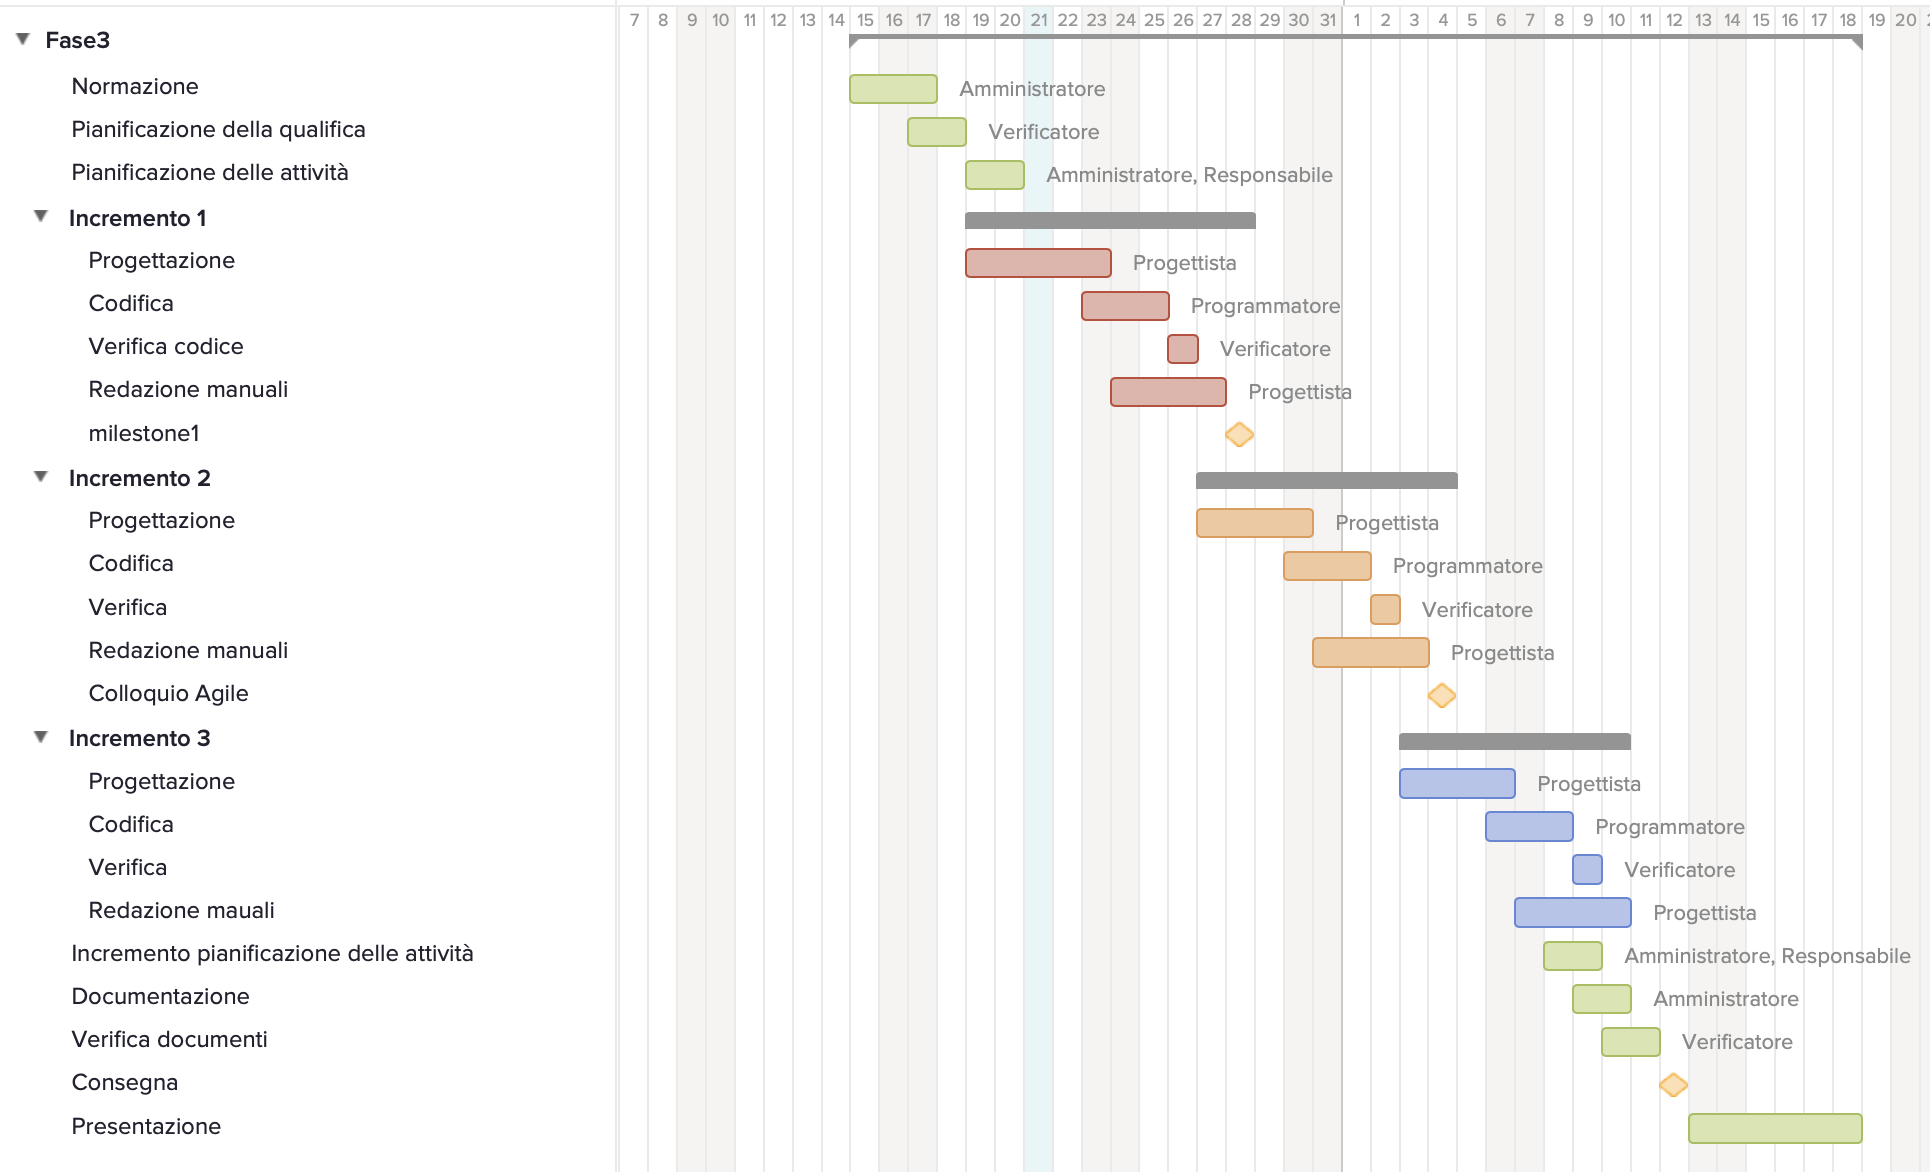
\includegraphics[scale=0.70]{images/fase3.png}
	\caption{Diagramma di Gantt riguardante la fase 3}
\end{figure}
	
\newpage	
\subsection{Periodo di Validazione (2019-04-13 - 2019-05-12)}
	Nella fase 4 vengono eseguiti i seguenti incrementi e attività:
\begin{itemize}
	\item Incremento 1
			\begin{itemize}
				\item normazione: modifiche alle \textit{NormeDiProgetto\_v3.0.0} secondo quanto segnalato alla Revisione di Qualifica. Si procede poi con il suo incremento;
				\item pianificazione della qualifica: modifiche al \textit{PianoDiQualifica\_v3.0.0} secondo quanto segnalato alla Revisione di qualifica. Si procede poi con il suo incremento;
				\item pianificazione delle attività: modifiche al \textit{PianoDiProgetto\_v3.0.0} secondo quanto segnalato alla Revisione di Qualifica;
			\end{itemize}
	\item Incremento 2 e Incremento 3
		\begin{itemize}
			\item progettazione di dettaglio: incremento al \textit{Product Baseline} con i requisiti indicati nella tabella 4;
			\item codifica: codifica degli incrementi effettuati durante la progettazione;
			\item redazione manuali: incrementi al \textit{ManualeUtente\_v1.0.0} e al \textit{ManualeSviluppatore\_v1.0.0} in base a quanto segnalato alla Revisione di Qualifica;
			\item verifica: verifica degli incrementi effettuati;
		\end{itemize}
	\item Incremento 4
		\begin{itemize}
			\item Documentazione;
			\item Verifica documentazione;
		\end{itemize}
	\item validazione e collaudo: vengono eseguiti i test di qualifica e il collaudo per il rilascio;
	\item preparazione alla presentazione;
	\item approvazione dei documenti da parte del responsabile. Sono pronti per il rilascio le \textit{NormeDiProgetto\_v4.0.0}, il \textit{PianoDiProgetto\_v4.0.0}, il \textit{PianoDiQualifica\_v4.0.0}, l'\textit{AnalisiDeiRequisiti\_v4.0.0} il
	\textit{ManualeUtente\_v2.0.0} e il \textit{ManualeSviluppatore\_v2.0.0};
\end{itemize}

\begin{tabularx}{\textwidth}{| c | c | }
	\rowcolor{LightBlue}
	\color{white}\bfseries Incremento 1 & 
	\color{white}\bfseries Incremento 2  \\[0.25cm]
	RDF22 & RDF3 \\ 
	RDF23 & RDF4 \\ 
	RDF24 & RDF5 \\ 
	RDF25 & RDF6 \\ 
	RDF26 & RDF7 \\ 
	RDF27 & RDF8 \\ 
	RDF28 & RDF10 \\ 
	RDF29 & RDF11 \\ 
	RDF30 & RDF12 \\ 
	RDF31 & RDF13 \\ 
	RDF32 & RDF14 \\ 
	RDF33 & RDF15 \\ 
	RDF34 & RDF16 \\ 
	RDF35 & RDF17 \\ 
	RDF36 & RDF18 \\
	RDF37 & RDF19\\
	RDF38 & RDF20 \\
	RDF39 & RDF21 \\
	RDF40 &  \\
	RDF41 &  \\
	RDF42 &  \\
	RDF43 &  \\
	RDF44 &  \\
		 \hline
		 \caption{Requisiti da soddisfare in fase 4}
\end{tabularx}

\begin{figure}[h]
	\centering
	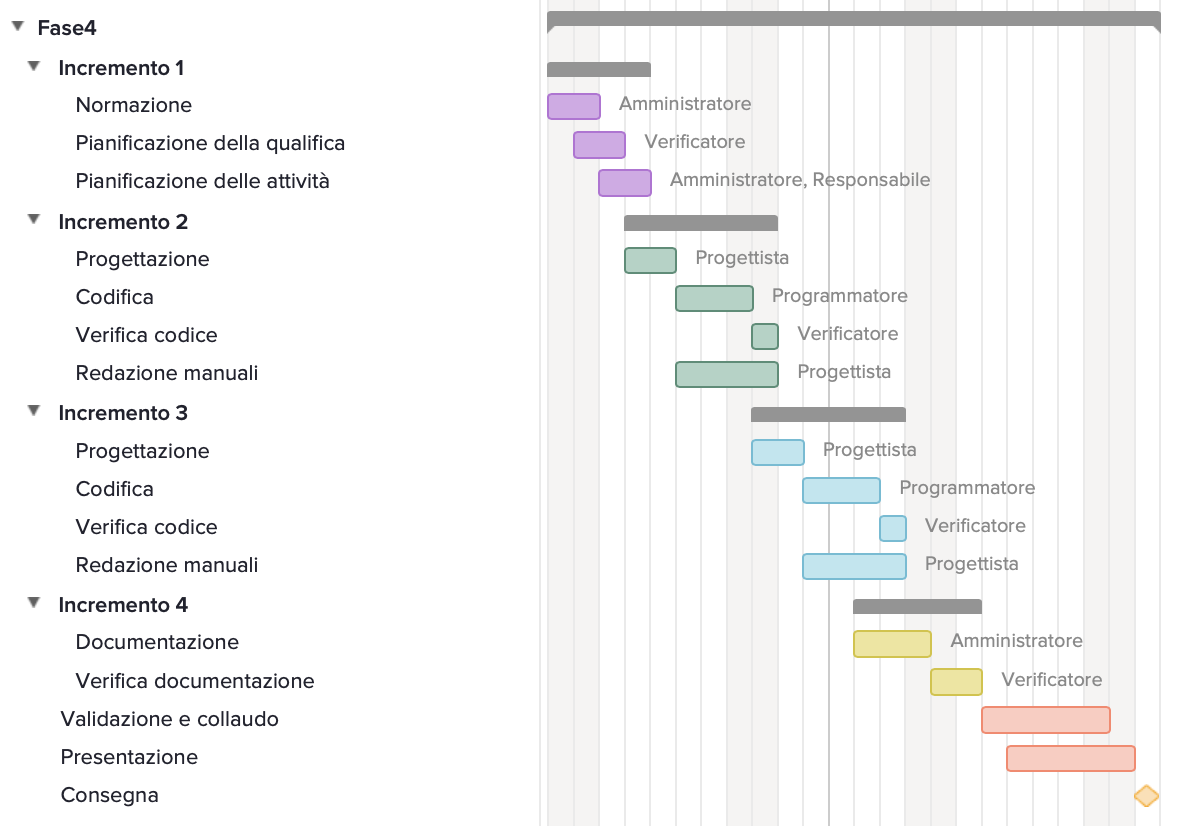
\includegraphics[scale=0.70]{images/fase4.png}
	\caption{Diagramma di Gantt riguardante la fase 4}
\end{figure}
	
\newpage
\subsection{Diagrammi di Gantt}
\begin{figure}[hbt!]
	\centering
	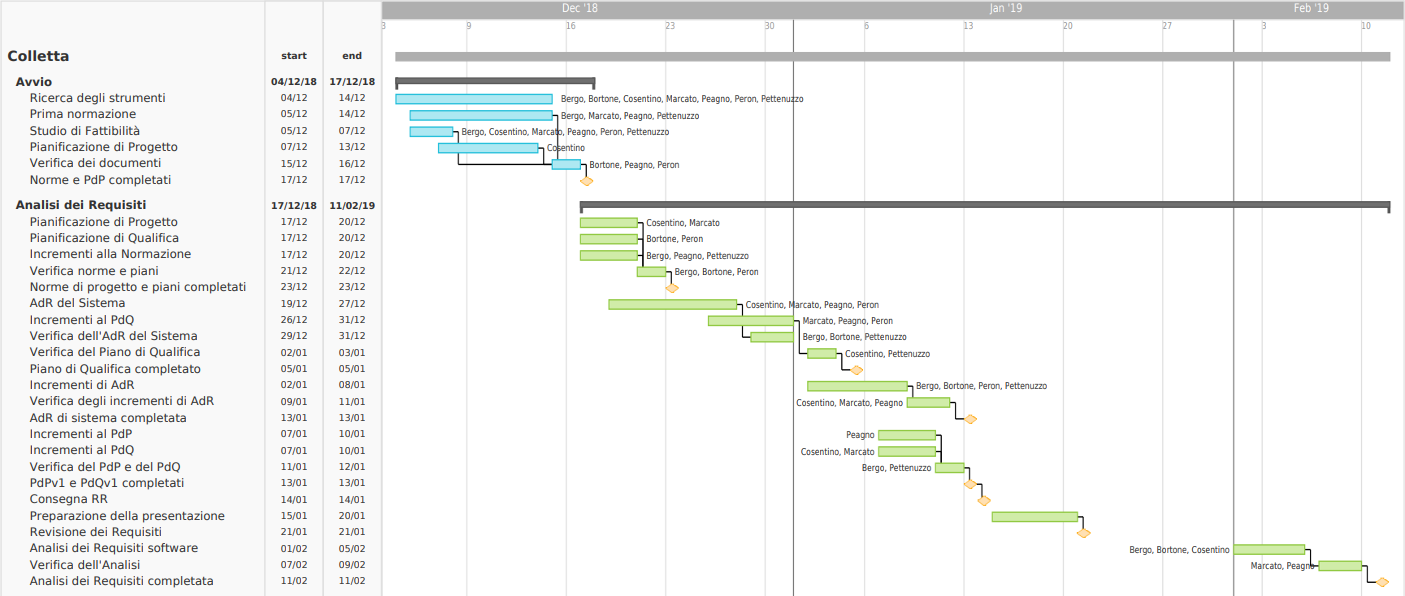
\includegraphics[scale=0.45,angle=90]{images/ganttan.png}
	\caption{Diagramma di Gantt per il periodo di avvio e di analisi}
\end{figure}

\newpage
\begin{figure}[hbt!]
	\centering
	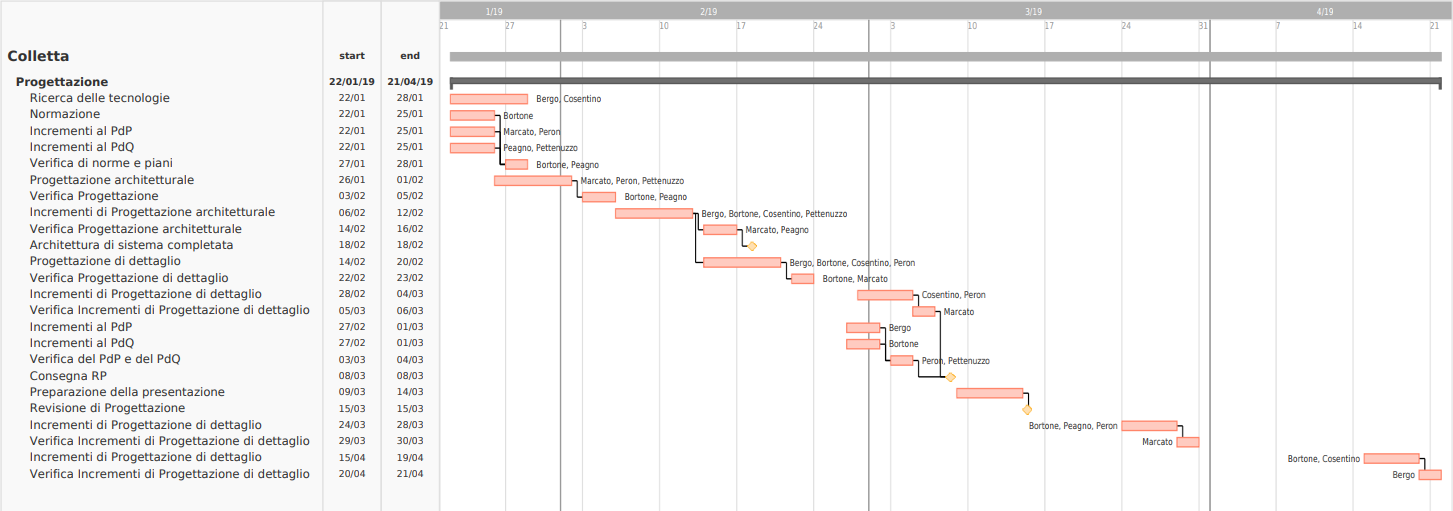
\includegraphics[scale=0.45,angle=90]{images/ganttprog.png}
	\caption{Diagramma di Gantt per il periodo progettazione}
\end{figure}

\newpage
\begin{figure}[hbt!]
	\centering
	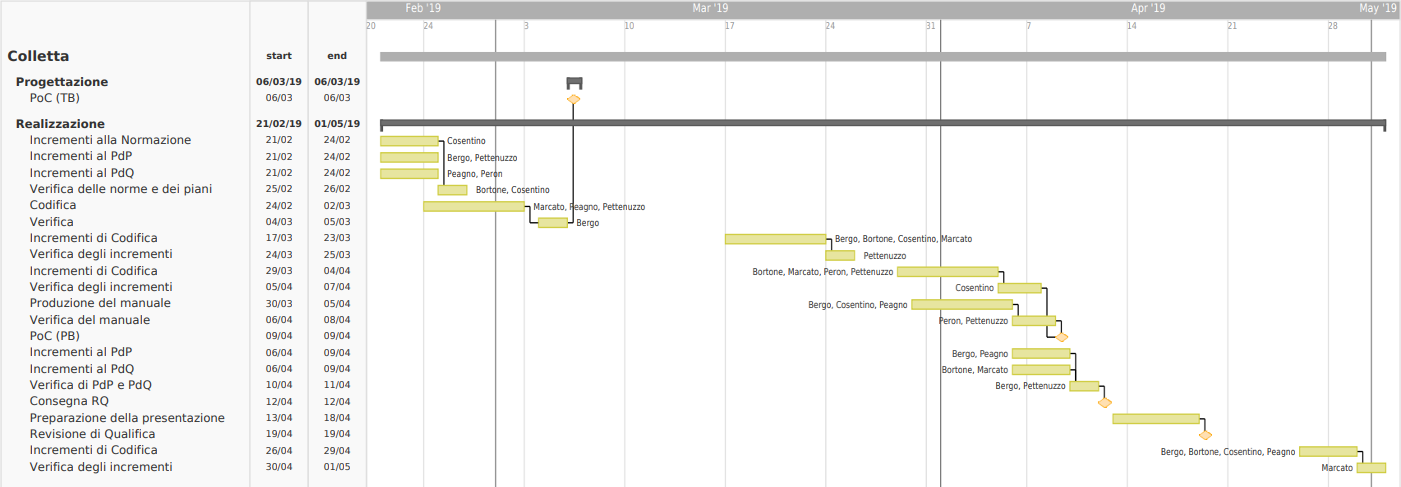
\includegraphics[scale=0.45, angle=90]{images/ganttreal.png}
	\caption{Diagramma di Gantt per il periodo di realizzazione}
\end{figure}

\newpage
\begin{figure}[hbt!]
	\centering
	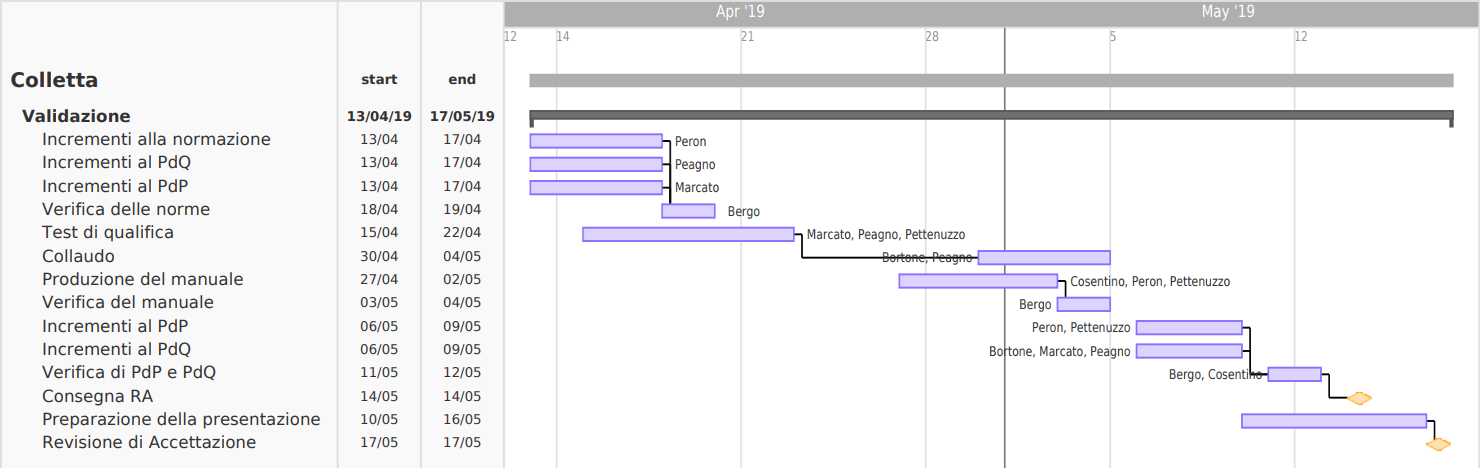
\includegraphics[scale=0.40, angle=90]{images/ganttval.png}
	\caption{Diagramma di Gantt per il periodo di validazione}
\end{figure}